\subsection{平行四边形的判定}\label{subsec:czjh1-4-4}

判定一个四边形是不是平行四边形,除根据定义来判定外,还有以下判定定理:

\begin{dingli}[平行四边形判定定理1]
    一组对边平行且相等的四边形是平行四边形。
\end{dingli}

\begin{wrapfigure}[8]{r}{5cm}
    \centering
    \begin{tikzpicture}
    \tkzDefPoints{0/0/B,  2.5/0/C, 3.3/1.5/D, 0.8/1.5/A}
    \tkzDrawPolygon(A,B,C,D)
    \tkzDrawSegment[dashed](A,C)
    \extkzLabelAngel[0.3](B,A,C){$1$}
    \extkzLabelAngel[0.5](A,C,B){$3$}
    \extkzLabelAngel[0.3](D,C,A){$2$}
    \extkzLabelAngel[0.5](C,A,D){$4$}
    \tkzLabelPoints[left](A,B)
    \tkzLabelPoints[right](C,D)
\end{tikzpicture}


    \caption{}\label{fig:czjh1-4-17}
\end{wrapfigure}

已知: 四边形 $ABCD$, $AB \pingxing CD$, $AB = CD$(图 \ref{fig:czjh1-4-17})。

求证: 四边形 $ABCD$ 是平行四边形。

\zhengming 连结 $AC$。

$\because$ \quad $AB \pingxing CD$,

$\therefore$ \quad $\angle 1 = \angle 2$。

又 $\because$ \quad $AB = CD$, $AC = CA$,

$\therefore$ \quad $\triangle ABC \quandeng \triangle CDA$。

$\therefore$ \quad $\angle 3 = \angle 4$。

$\therefore$ \quad $BC \pingxing AD$。

所以四边形 $ABCD$ 是平行四边形。

“平行且等于” 用符号 “$\pxqdy$”  表示。
如图 \ref{fig:czjh1-4-17}, $AB = DC$, 且 $AB \pingxing DC$, 可以记作 $AB \pxqdy DC$,
读作 “$AB$ 且等于 $DC$”。

和定理 1 相类似,利用全等三角形,容易证明平行四边形判定定理 2、3。

\begin{dingli}[平行四边形判定定理2]
    两组对边分别相等的四边形是平行四边形。
\end{dingli}

\begin{dingli}[平行四边形判定定理3]
    对角线互相平分的四边形是平行四边形。
\end{dingli}



\liti 已知: $\pxsbx ABCD$ 中, $E$、$F$ 分别是边 $AD$、$BC$ 的中点(图 \ref{fig:czjh1-4-18})。

求证: $EB = DF$。

\zhengming $\because$ \quad 四边形 $ABCD$ 是平行四边形,

$\therefore$ \quad $AD \pxqdy BC$ (平行四边形对边平行且相等)。

\begin{enhancedline}
$\because$ \quad $ED = \exdfrac{1}{2} AD$, $BF = \exdfrac{1}{2} BC$,

$\therefore$ \quad $ED \pxqdy BF$。
\end{enhancedline}

$\therefore$ \quad 四边形 $EBFD$ 是平行四边形(一组对边平行并且相等的四边形是平行四边形)。

$\therefore$ \quad $EB = DF$ (平行四边形的对边相等)。


\begin{figure}[htbp]
    \centering
    \begin{minipage}[b]{7cm}
        \centering
        \begin{tikzpicture}
    \tkzDefPoints{0/0/B,  2.5/0/C, 3.3/1.5/D, 0.8/1.5/A}
    \tkzDefMidPoint(A,D)  \tkzGetPoint{E}
    \tkzDefMidPoint(B,C)  \tkzGetPoint{F}
    \tkzDrawPolygon(A,B,C,D)
    \tkzDrawSegments(B,E  D,F)
    \tkzLabelPoints[left](A,B)
    \tkzLabelPoints[right](C,D)
    \tkzLabelPoints[above](E)
    \tkzLabelPoints[below](F)
\end{tikzpicture}


        \caption{}\label{fig:czjh1-4-18}
    \end{minipage}
    \qquad
    \begin{minipage}[b]{7cm}
        \centering
        \begin{tikzpicture}
    \tkzDefPoints{0/0/B,  2.5/0/C, 1.5/1.5/A}
    \tkzDrawSegment(B,C)
    \tkzLabelPoints[above](A)
    \tkzLabelPoints[below](B,C)

    % 思路 1
    % 1.1
    \tkzDrawSegment(A,B)
    % 1.2
    \tkzInterCC[with nodes](A,B,C)(C,A,B)  \tkzGetFirstPoint{D}
    \tkzLabelPoints[right](D)
    % 1.3
    \tkzCompasss(A,D  C,D)
    \tkzDrawSegments(A,D  C,D)

    % 思路 2
    % 2.1
    \tkzDrawSegment[red](A,C)
    % 2.2
    \tkzInterCC[with nodes](A,B,C)(B,A,C)  \tkzGetSecondPoint{E}
    \tkzLabelPoints[left](E)
    % 2.3
    \tkzCompasss(A,E  B,E)
    \tkzDrawSegments[red](A,E  B,E)
\end{tikzpicture}


        \caption{}\label{fig:czjh1-4-19}
    \end{minipage}
\end{figure}


\liti 已知: 线段 $BC$ 和直线 $BC$ 外一点 $A$ (图 \ref{fig:czjh1-4-19})。

求作: 以 $A$ 为一顶点, 以线段 $BC$ 为一边的平行四边形。

分析: 如果连结 $AB$, 那么平行四边形的两边已确定,根据平行四边形对边相等就可以确定另一个顶点。

\zuofa 1. 连结 $AB$。

2. 分别以 $A$、$C$ 为圆心, 以 $BC$、$AB$ 为半径作弧,两弧相交于点 $D$。

3. 连结 $AD$、$CD$。

四边形 $ABCD$ 就是所求的平行四边形。


\zhengming $\because$ \quad $AD = BC$, $DC = AB$,

$\therefore$ \quad 四边形 $ABCD$ 是平行四边形(两组对边分别相等的四边形是平行四边形)。

$\because$ \quad $\pxsbx ABCD$ 的一边是 $BC$, 一个顶点是 $A$,

$\therefore$ \quad 四边形 $ABCD$ 就是所求的平行四边形。

讨论: 如果连结 $AC$, 同理可作四边形 $AEBC$, 它也是所求的平行四边形。此题有两个解。


\begin{lianxi}

\xiaoti{求证:\zhongdian{两组对角分别相等的四边形是平行四边形。}}

\xiaoti{把两个全等的三角形,按不同的方法拼成四边形,可以拼成几个不同的四边形,它们都是平行四边形吗?为什么?}

\xiaoti{已知: $\pxsbx ABCD$, $E$ 是 $AB$ 的中点, $F$ 是 $CD$ 的中点。
    求证: $EF = BC$。
}

\xiaoti{延长 $\triangle ABC$ 的中线 $AD$ 至 $E$, 使 $DE = AD$。
    求证: 四边形 $ABEC$ 是平行四边形。
}

\end{lianxi}


